\begin{figure}[H]
\centering
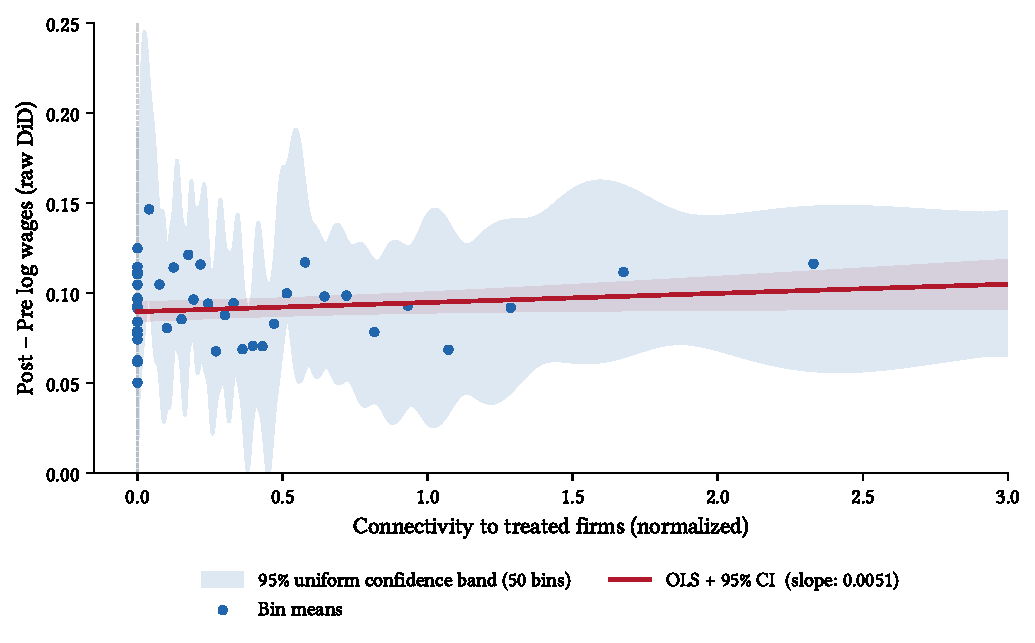
\includegraphics[width=0.75\textwidth]{linearity_fig3_binsreg_corrected.pdf}
\caption{Dose--Response Relationship Between Connectivity and Wages: Nonparametric Evidence}
\label{fig:linearity_binsreg_corrected}
\begin{minipage}{0.75\textwidth}
    \vspace{0.3em}
    \footnotesize
    \textit{Notes:} This figure presents nonparametric evidence on the shape of the dose--response relationship between pre-treatment connectivity to treated firms and the post-reform change in log wages. The sample consists of spillover-sample establishments with zero prior union contract coverage that belong to a balanced panel over 2009--2016. The $x$-axis measures pre-treatment connectivity, defined as worker flows from establishment $i$ to treated firms normalized by establishment $i$'s total employment ($\text{totaltreat\_pw\_n}$), further normalized by the 90th percentile of the connectivity distribution in 2009. The $y$-axis is the firm-level difference-in-differences estimand: the difference between the post-reform (2012--2016) and pre-reform (2009--2011) averages of log December wages.

    Dots and the shaded region represent, respectively, the bin-mean estimates and the 95\% uniform confidence band from a covariate-adjusted binscatter with 50 bins, implemented following \citet{Cattaneo2024}. Critically, covariate adjustment is performed internally by the estimator rather than through prior residualization of the outcome and running variable, which is the approach advocated by \citet{Cattaneo2024} to avoid distortions in shape and support that arise under the standard (incorrect) residualized binscatter when the true conditional mean is nonlinear. Specifically, the estimator projects out a vector of controls $w_i$ consisting of indicator variables for two-digit industry, base negotiation month, microregion, and quartile bins of pre-reform log wages, log employment, and per-worker worker flows (2007--2011), implementing the semi-linear partial-mean estimator of \citet{Cattaneo2024} (their equation~3). The solid red line and shaded band report the OLS estimate and its 95\% confidence interval from a regression of the raw difference-in-differences on connectivity and the full control vector $w_i$, evaluated at the sample mean of $w_i$.

    The 95\% uniform confidence band encompasses the OLS line throughout the support of connectivity, indicating that the data are consistent with a linear dose--response relationship. The OLS slope of $0.005$ is nearly identical to the slope obtained from the residualized binscatter ($0.005$), validating the use of the residualized specification as an approximation in this setting.
\end{minipage}
\end{figure}
